% Open Orders by MSA team review: the Part 2 questions as a printed sheet to write on during the meeting.
% One 11 x 17 landscape sheet (ledger, 17 x 11 in) drawn in TikZ, in the house style of open-orders-team-review.tex.
% The questions are the ones on the agenda sheet of open-orders-team-review.tex ("Where does the data need to go?",
% The data, The deck; the data first, as on the agenda), word for word (Snowflake capitalised); keep the two in step. The third column is blank, for the owner's own questions.
% Laid out on a 12 x 7.5 in grid and scaled by 4/3 to fill the 16 x 10 in drawing area (writing lines 0.35 in apart).
% Build: ./build.sh source/open-orders-intake-inventory/open-orders-meeting-questions.tex
\documentclass[10pt]{article}
\usepackage[paperwidth=17in, paperheight=11in, margin=0.5in]{geometry}
\usepackage[T1]{fontenc}
\usepackage{lmodern}
\usepackage{microtype}
\usepackage{xcolor}
\usepackage{tikz}
\usetikzlibrary{calc}
\usepackage[hidelinks, pdftitle={Open Orders by MSA: Meeting Questions}, pdfauthor={Gust F.}]{hyperref}
\pagestyle{empty}
\setlength{\parindent}{0pt}
\hyphenpenalty=10000
\exhyphenpenalty=10000
\definecolor{headgreen}{HTML}{548235}
\tikzset{every node/.style={font=\sffamily\small, inner sep=5pt}}
% column header: #1 x, #2 text
\newcommand{\colhead}[2]{%
  \draw[line width=0.5pt, fill=headgreen] (#1,6.22) rectangle (#1+3.7,6.5);
  \node[anchor=west, text=white, font=\sffamily\bfseries\normalsize] at (#1,6.36) {#2};}
% writing block: #1 x, #2 top, #3 bottom, #4 number, #5 question (blank: a "Q" line to write one)
% writing lines every 0.26 in from below the question, and an Owner line at the foot of the block
\newcommand{\qblock}[5]{%
  \draw[line width=0.5pt] (#1,#2) rectangle (#1+3.7,#3);
  \node[fill=headgreen, text=white, font=\sffamily\bfseries\small, inner sep=0pt, minimum size=0.22in]
    at (#1+0.21,#2-0.21) {#4};
  \if\relax\detokenize{#5}\relax
    \node[anchor=west, font=\sffamily\bfseries\small, inner sep=0pt] at (#1+0.4,#2-0.25) {Q};
    \draw[line width=0.3pt] (#1+0.58,#2-0.3) -- (#1+3.58,#2-0.3);
    \def\qfirst{0.56}%
  \else
    \node[anchor=north west, text width=3.1in, inner sep=0pt, font=\sffamily\bfseries\small] at (#1+0.42,#2-0.12) {#5};
    \def\qfirst{0.66}%
  \fi
  \node[anchor=south west, font=\sffamily\footnotesize, inner sep=0pt] at (#1+0.12,#3+0.17) {Owner};
  \draw[line width=0.3pt] (#1+0.62,#3+0.14) -- (#1+3.58,#3+0.14);
  \pgfmathsetmacro{\qlast}{#2-#3-0.38}%
  \pgfmathtruncatemacro{\qn}{floor((\qlast-\qfirst)/0.26)}%
  \foreach \i in {0,...,\qn} {
    \pgfmathsetmacro{\d}{\qfirst+0.26*\i}%
    \draw[line width=0.3pt] (#1+0.12,#2-\d) -- (#1+3.58,#2-\d);
  }}
% title block, one row in the bottom right corner: #1 title, #2 sheet
\newcommand{\titleblock}[2]{%
  \draw[line width=0.5pt] (5.7,0) -- (5.7,0.42) -- (12,0.42);
  \foreach \x in {7.3, 8.95, 9.5, 9.95, 10.75, 11.45} \draw[line width=0.5pt] (\x,0) -- (\x,0.42);
  \foreach \x/\label/\value in {5.7/Title/#1, 7.3/Project/Open Orders by MSA, 8.95/Macro/v2.4, 9.5/Rev./2,
                                9.95/Date/2026-10-14, 10.75/Drawn/Gust F., 11.45/Sheet/#2} {
    \node[anchor=north west, inner sep=0pt, font=\sffamily\fontsize{7}{8}\selectfont] at (\x+0.07,0.36) {\label};
    \node[anchor=south west, inner sep=0pt, font=\sffamily\bfseries\footnotesize] at (\x+0.07,0.07) {\value};
  }}

\begin{document}
\noindent
\scalebox{1.333333}{%
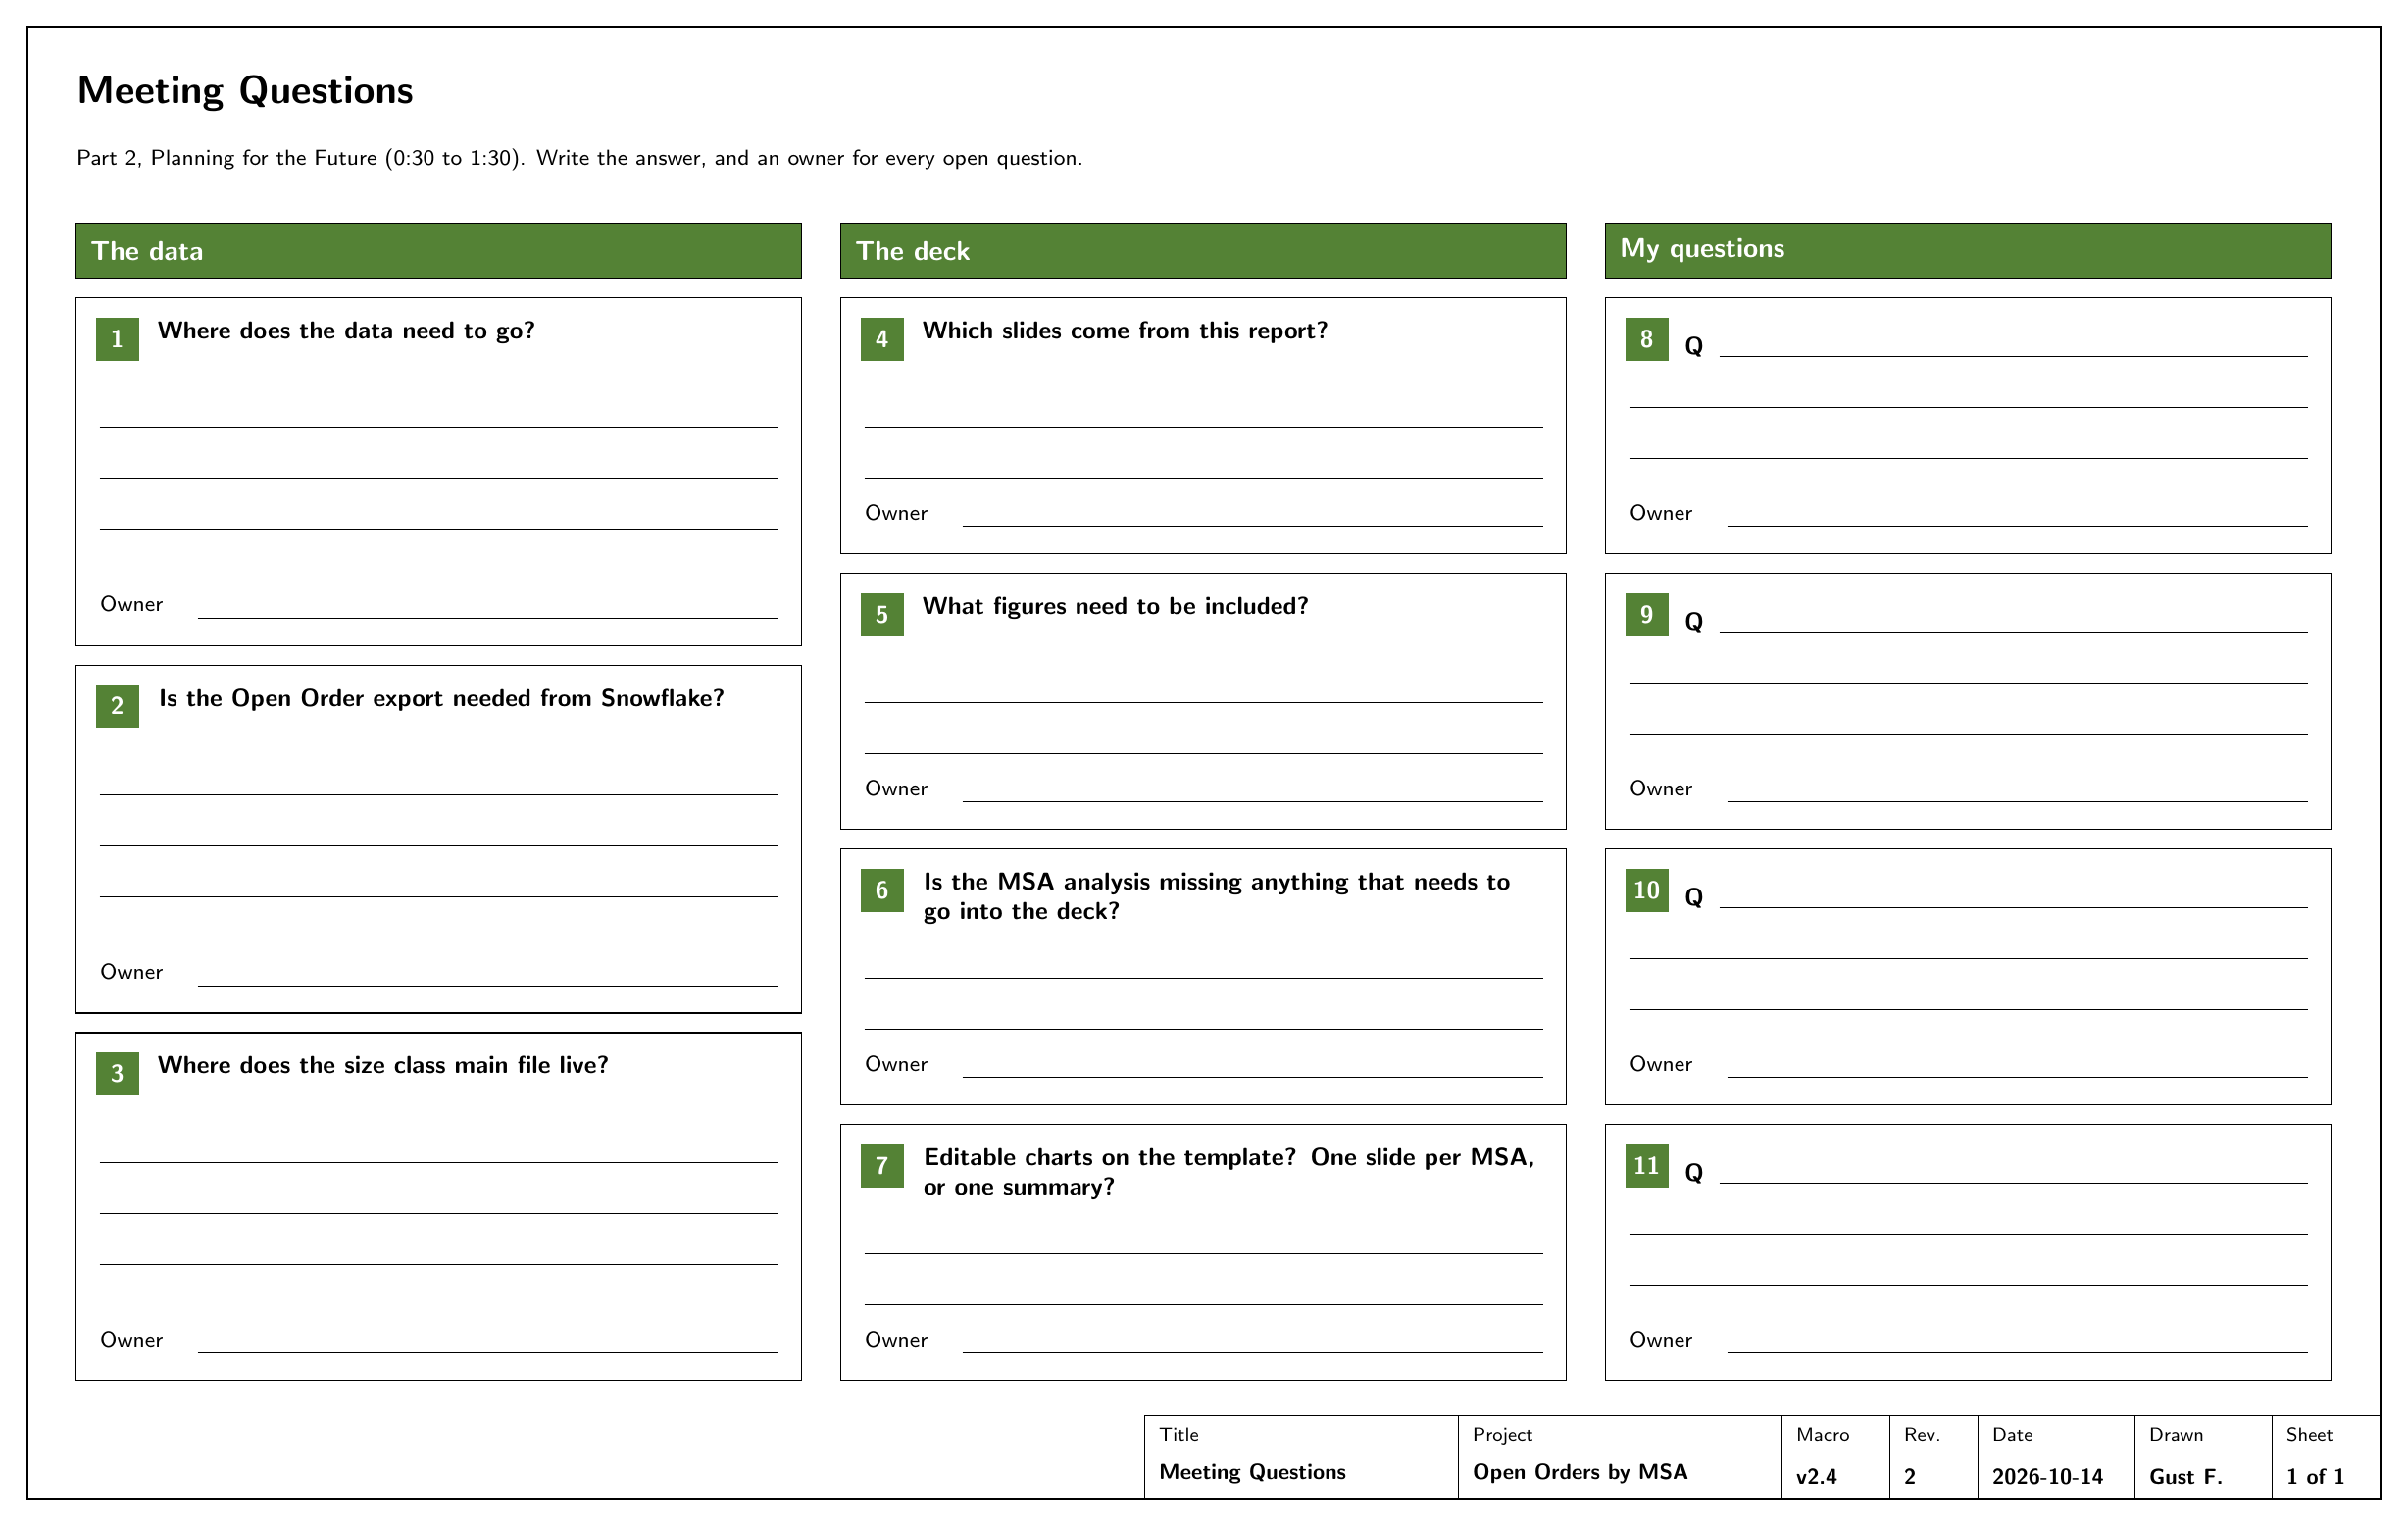
\begin{tikzpicture}[x=1in, y=1in]
\useasboundingbox (0,0) rectangle (12,7.5);
\draw[line width=0.8pt] (0,0) rectangle (12,7.5);

\node[anchor=north west, inner sep=0pt, font=\sffamily\bfseries\fontsize{14}{16}\selectfont]
  at (0.25,7.25) {Meeting Questions};
\node[anchor=north west, inner sep=0pt, font=\sffamily\footnotesize] at (0.25,6.88)
  {Part 2, Planning for the Future (0:30 to 1:30). Write the answer, and an owner for every open question.};

% ---------------------------------------------------------------- the data: 3 blocks of 1.773 in, 0.1 in apart
\colhead{0.25}{The data}
\qblock{0.25}{6.12}{4.3467}{1}{Where does the data need to go?}
\qblock{0.25}{4.2467}{2.4733}{2}{Is the Open Order export needed from Snowflake?}
\qblock{0.25}{2.3733}{0.6}{3}{Where does the size class main file live?}

% ---------------------------------------------------------------- the deck: 4 blocks of 1.305 in, 0.1 in apart
\colhead{4.15}{The deck}
\qblock{4.15}{6.12}{4.815}{4}{Which slides come from this report?}
\qblock{4.15}{4.715}{3.41}{5}{What figures need to be included?}
\qblock{4.15}{3.31}{2.005}{6}{Is the MSA analysis missing anything that needs to go into the deck?}
\qblock{4.15}{1.905}{0.6}{7}{Editable charts on the template? One slide per MSA, or one summary?}

% ---------------------------------------------------------------- my questions: 4 blank blocks
\colhead{8.05}{My questions}
\qblock{8.05}{6.12}{4.815}{8}{}
\qblock{8.05}{4.715}{3.41}{9}{}
\qblock{8.05}{3.31}{2.005}{10}{}
\qblock{8.05}{1.905}{0.6}{11}{}

\titleblock{Meeting Questions}{1 of 1}
\end{tikzpicture}}
\end{document}
